\section{Zephyr RTOS}
As we seen just before, RTOS may be very usefull to create complex programs on CPUs.
Since we're using Zephyr, let's dig a bit deeper into this RTOS.

\subsection{Configuration}
As we seen previously, Zephyr isn't based on pure code to configure the device. It used
a lot of others files, including devicetrees to describe the hardware.

This image represent the different steps to build an executable image for our chip
\begin{figure}[!hbt]
    \centering
    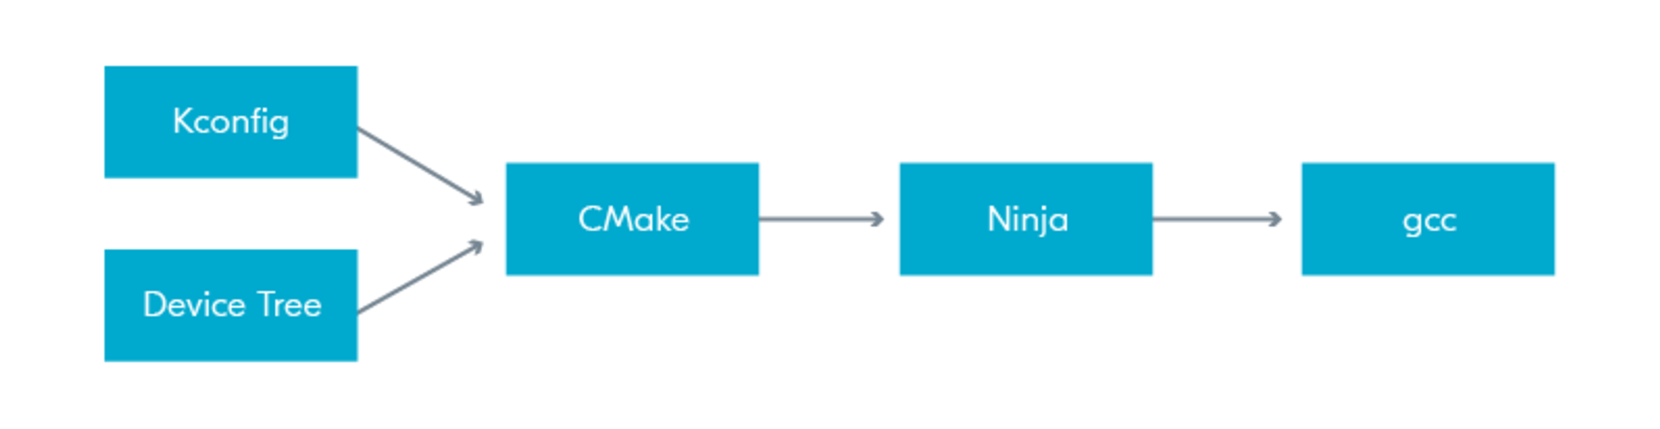
\includegraphics[width=\SchematicWidth]{\Images/Zephyr/ZephyrBuild.eps}
    \caption{Thread management on the Zephyr RTOS}
\end{figure}
\FloatBarrier

In this image, KConfig refer to the software configuration files, that include
drivers selections and so. This file is linked to the devicetree, because to
exploit a peripheral, we need to enable it in hardware, but we also need the associated
drivers with it.

To give an example, this kind of files look like :
\inputminted[linenos, firstline=32, lastline=70]{kconfig}{\Conf/prj.conf}

Thats basically a list of variable that we set to enable, or disable a software driver.

\subsection{Tasks management}
Zephyr does the task management in a different way other RTOS would. It is not bound to
the fixed interval timer that would trigger a scheduling every period. This RTOS use the
task as self-scheduling.

\begin{figure}[!hbt]
    \centering
    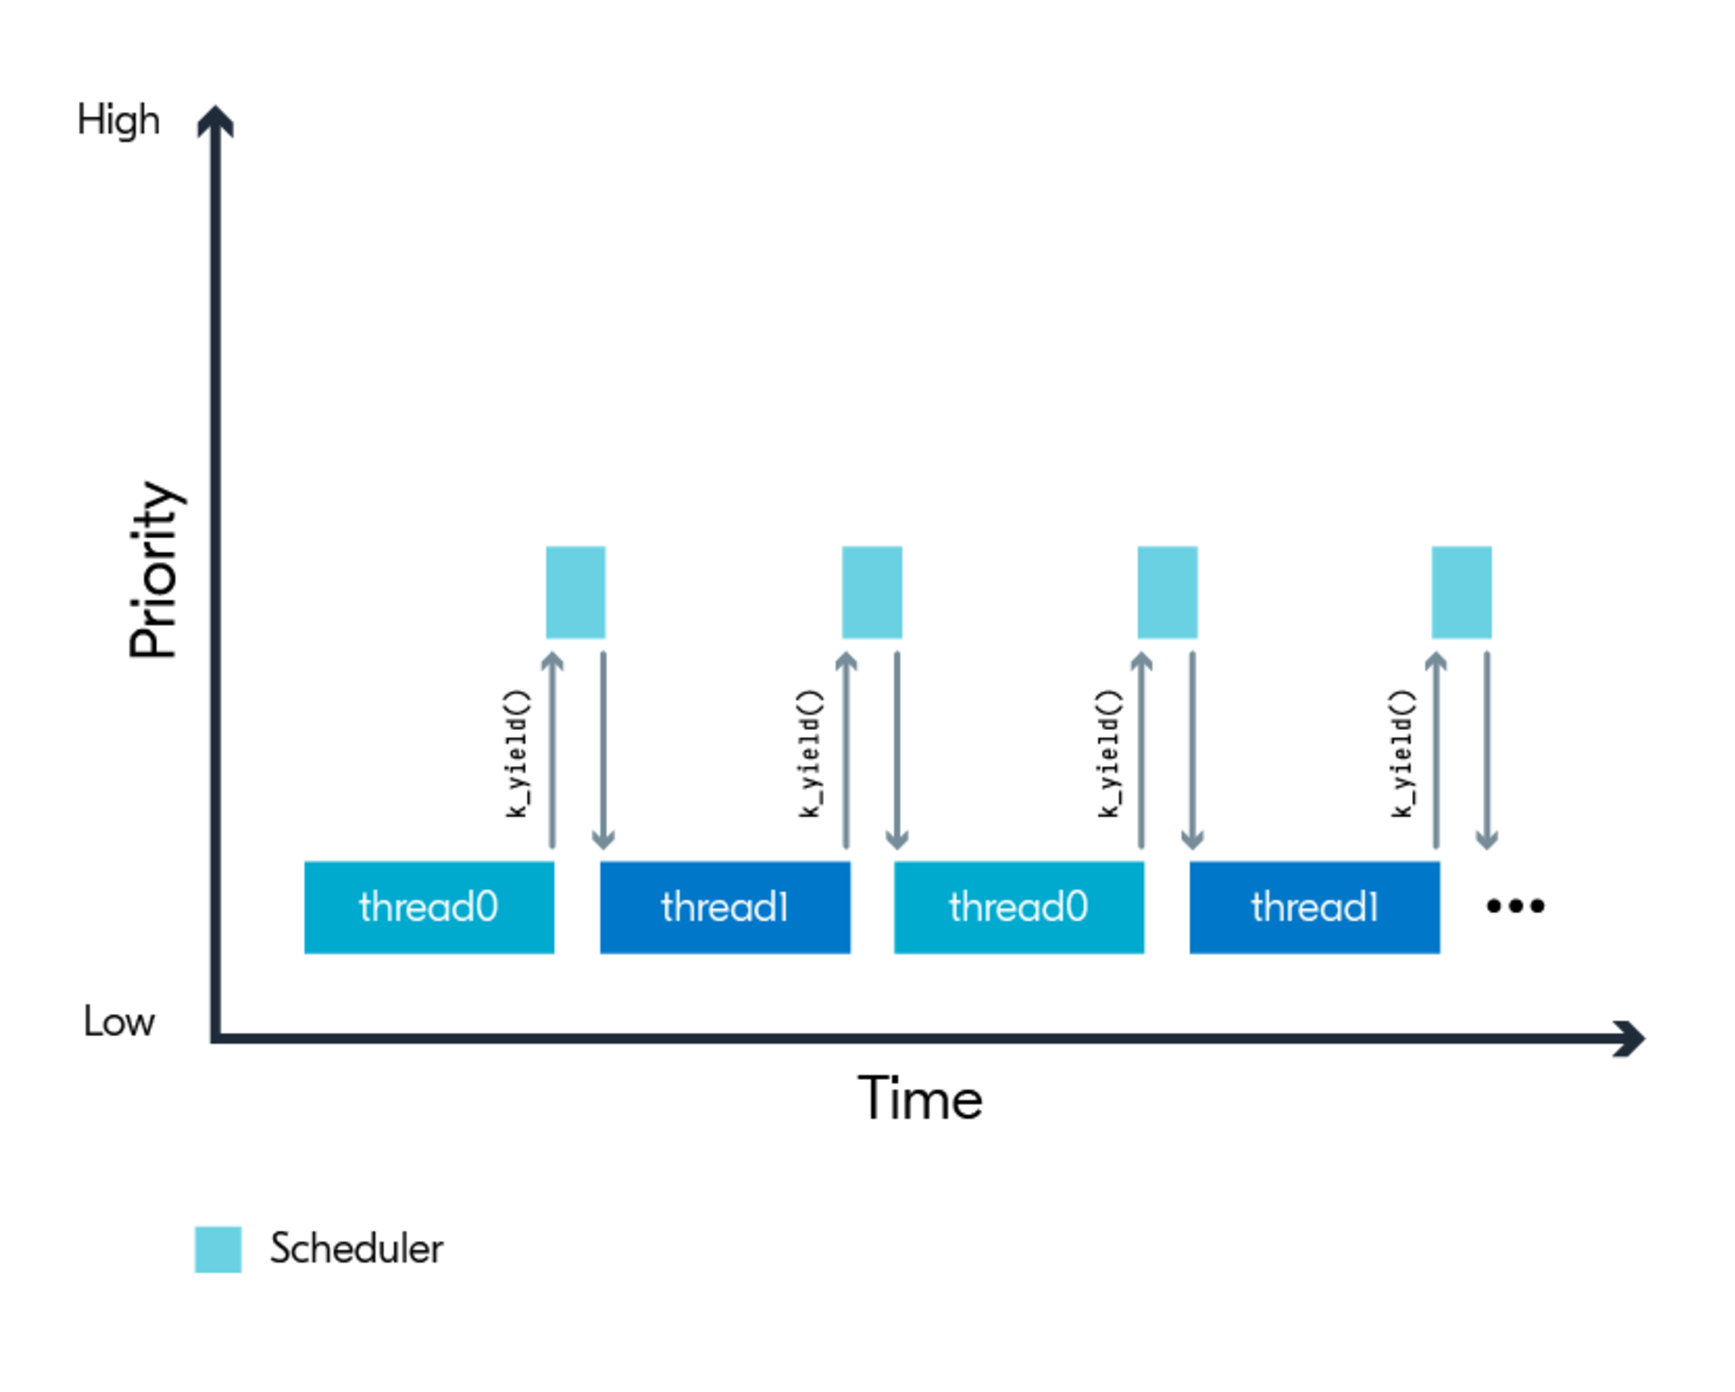
\includegraphics[width=\SchematicWidth]{\Images/Zephyr/ThreadMGNT.eps}
    \caption{Build chain for Zephyr RTOS}
\end{figure}
\FloatBarrier

As we may see on this image, that came from the Nordic training center \cite{NordicFundamentals}
and \cite{NordicAdvanced} courses, the scheduler is called once a task enter a delay state, or
yield itself.

On another hand, the RTOS include a safety timer, set to ten milliseconds that will force the
scheduler to be called. This ensure, even if a task enter an infinite loop, or crash, that
the others tasks wont crash.

\subsection{Final words}
To conclude on this RTOS part, we've seen the most basic concepts, but that's enough to
understand how our project is build, and how code interract with other code.

To sum up, Zephyr is an RTOS, used to manage a lot of different things on the project,
from the most basic configuration of the hardware to the tasks management during the
execution.
